\documentclass[../Orator]{subfiles}
\begin{document}

The FitzHugh-Nagumo model can be written in many ways, one of which is as follows.

\begin{equation}
    \dot{V}=V-\frac{V^{3}}{3}-W+I
\end{equation}

\begin{equation}
    \dot{W}=\phi (V+a-bW)
\end{equation}

The original values for the constants are \(a=0.7\), \(b=0.8\), and \(\phi=0.08\) \cite{}. For these values, the \glspl{gls:nullcline} look like \Cref{fig:nullclines-original}. 

\begin{figure}[ht]
    \centering
    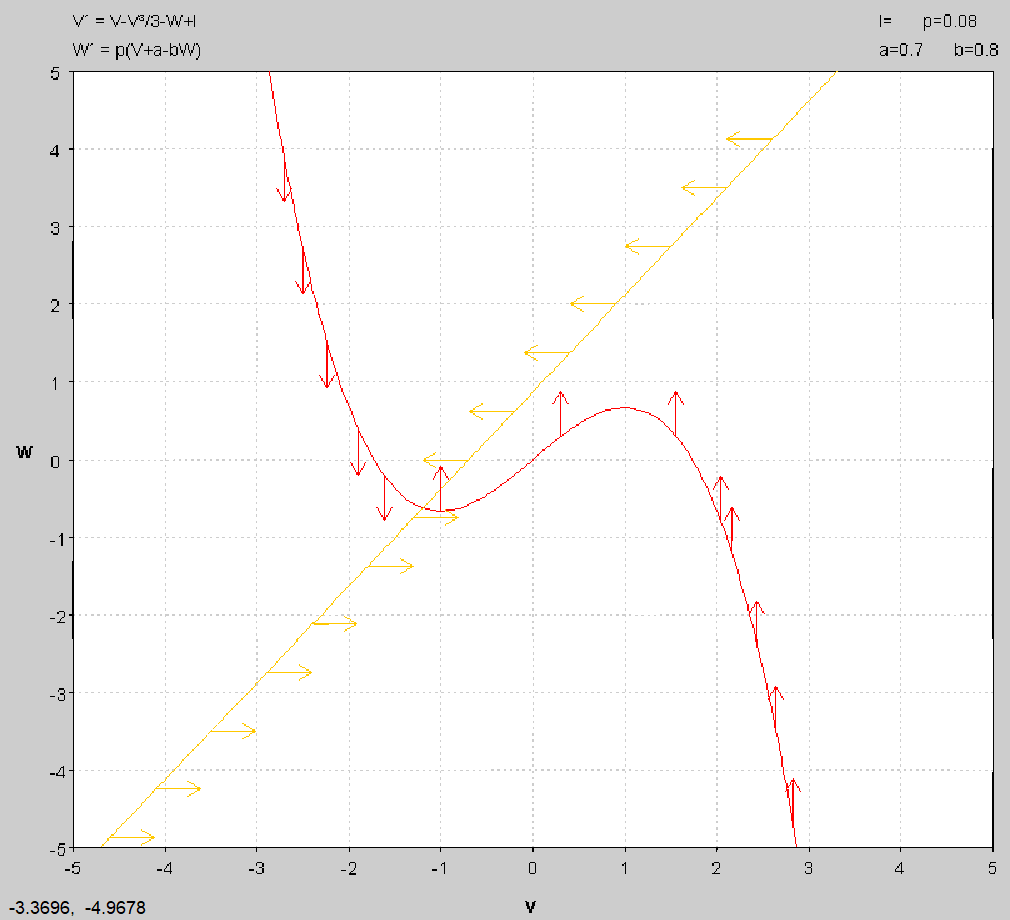
\includegraphics[width=0.7\textwidth]{Pictures/Alex/Nullclines - original.PNG}
    \caption{\Glspl{gls:nullcline} for \(I=0\), \(a=0.7\), \(b=0.8\), and \(\phi=p=0.08\)}
    \label{fig:nullclines-original}
\end{figure}

As can be seen in \Cref{fig:nullclines-original} there is only one \gls{gls:equil}. This is located at \((-1.1994, -0.62426)\). This is a \gls{gls:spiral}. 

It is also possible for the model to have three \glspl{gls:equil}. This is for example the case if \(b\) is changed to \(-0.8\). This can be seen in \Cref{fig:nullclines-negative}.

\begin{figure}[ht]
    \centering
    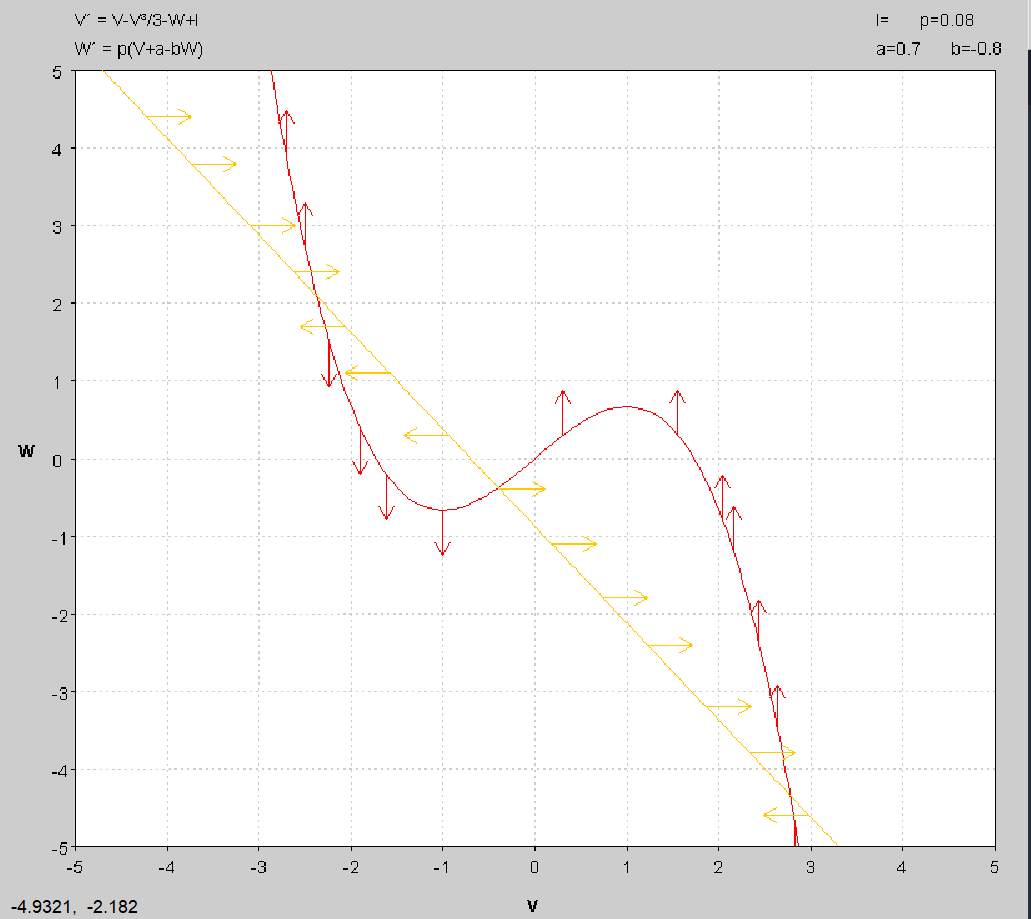
\includegraphics[width=0.7\textwidth]{Pictures/Alex/Nullclines - negative.PNG}
    \caption{\glspl{gls:nullcline} for \(I=0\), \(a=0.7\), \(b=-0.8\), and \(\phi=p=0.08\)}
    \label{fig:nullclines-negative}
\end{figure}

Here the \glspl{gls:equil} are at \((-2.376, 2.0949)\), \((-0.39825, -0.37719)\), and \((2.7742, -4.3428)\). The first and last are \glspl{gls:saddle} and the middle is a \gls{gls:nodal}.

The parametric solution to this system is \(V+a=bW\) and \(W=V-V^3/3+I\).

This change from one to three \glspl{gls:equil} changes at b>0. 

\begin{comment}
    Why do we have 1/3 fixed points?
        Because of the slope of W???
        But why in a biological sense?
\end{comment}

\end{document}